\newpage
\section{\textbf{THIẾT KẾ HỆ THỐNG}}

\subsection{Tổng quan hệ thống}

\begin{figure}[H]
	\centering
	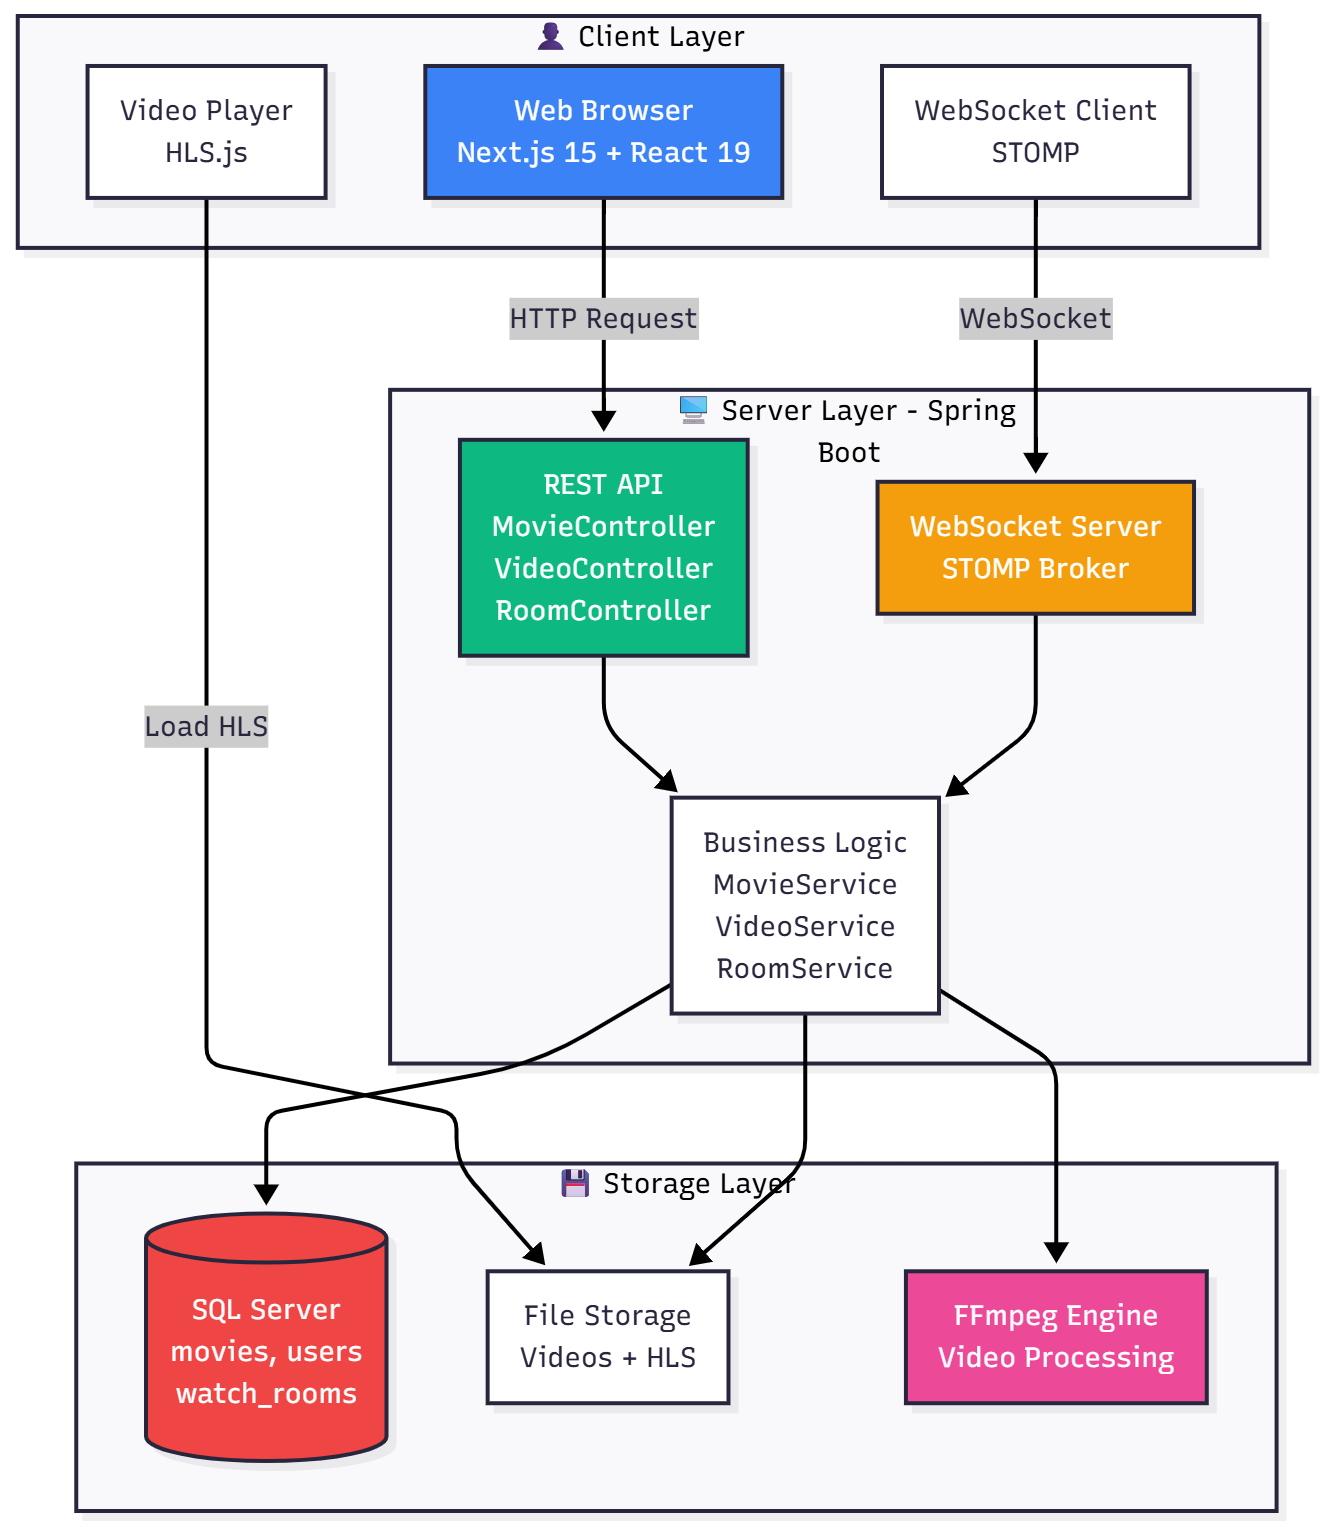
\includegraphics[width=1\textwidth]{image/mermaid/tongquahethong.png}
	\caption{Tổng quan hệ thống NicePhim}
	\label{fig:tongquahethong}
\end{figure}

\subsection{Luồng xử lý video}

\begin{figure}[H]
	\centering
	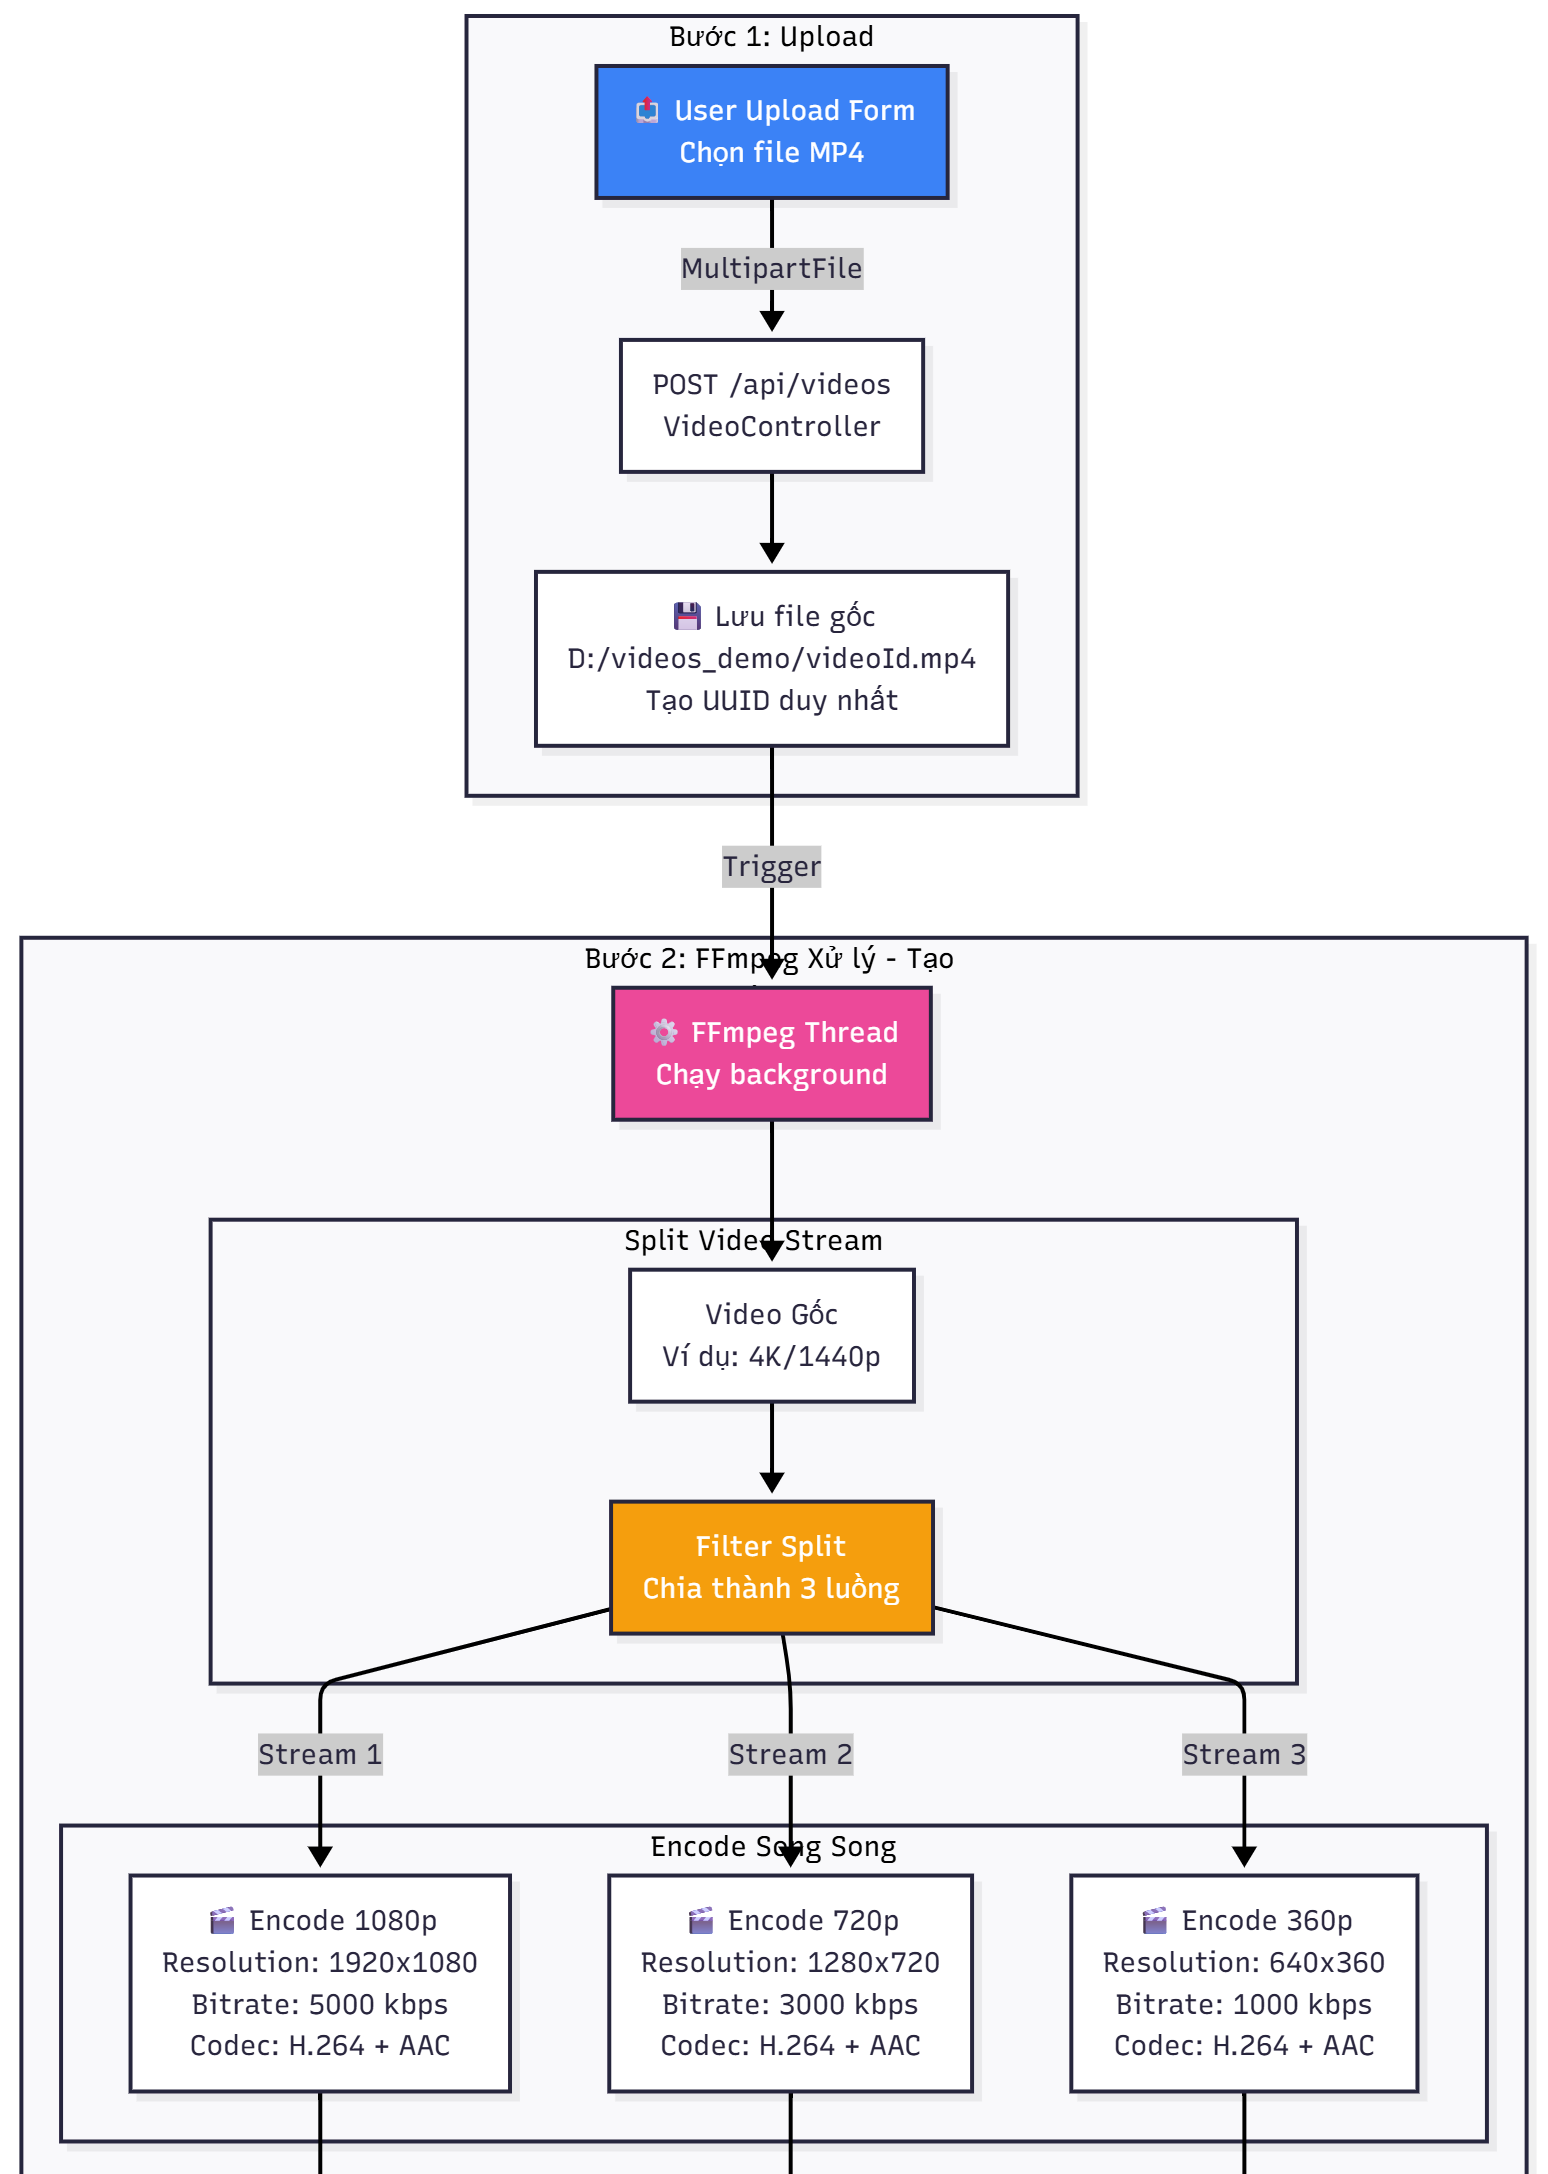
\includegraphics[width=1\textwidth]{image/mermaid/luongxulyvideo.png}
	\caption{Luồng xử lý video trong hệ thống NicePhim}
	\label{fig:luongxulyvideo}
\end{figure}

\begin{figure}[H]
	\centering
	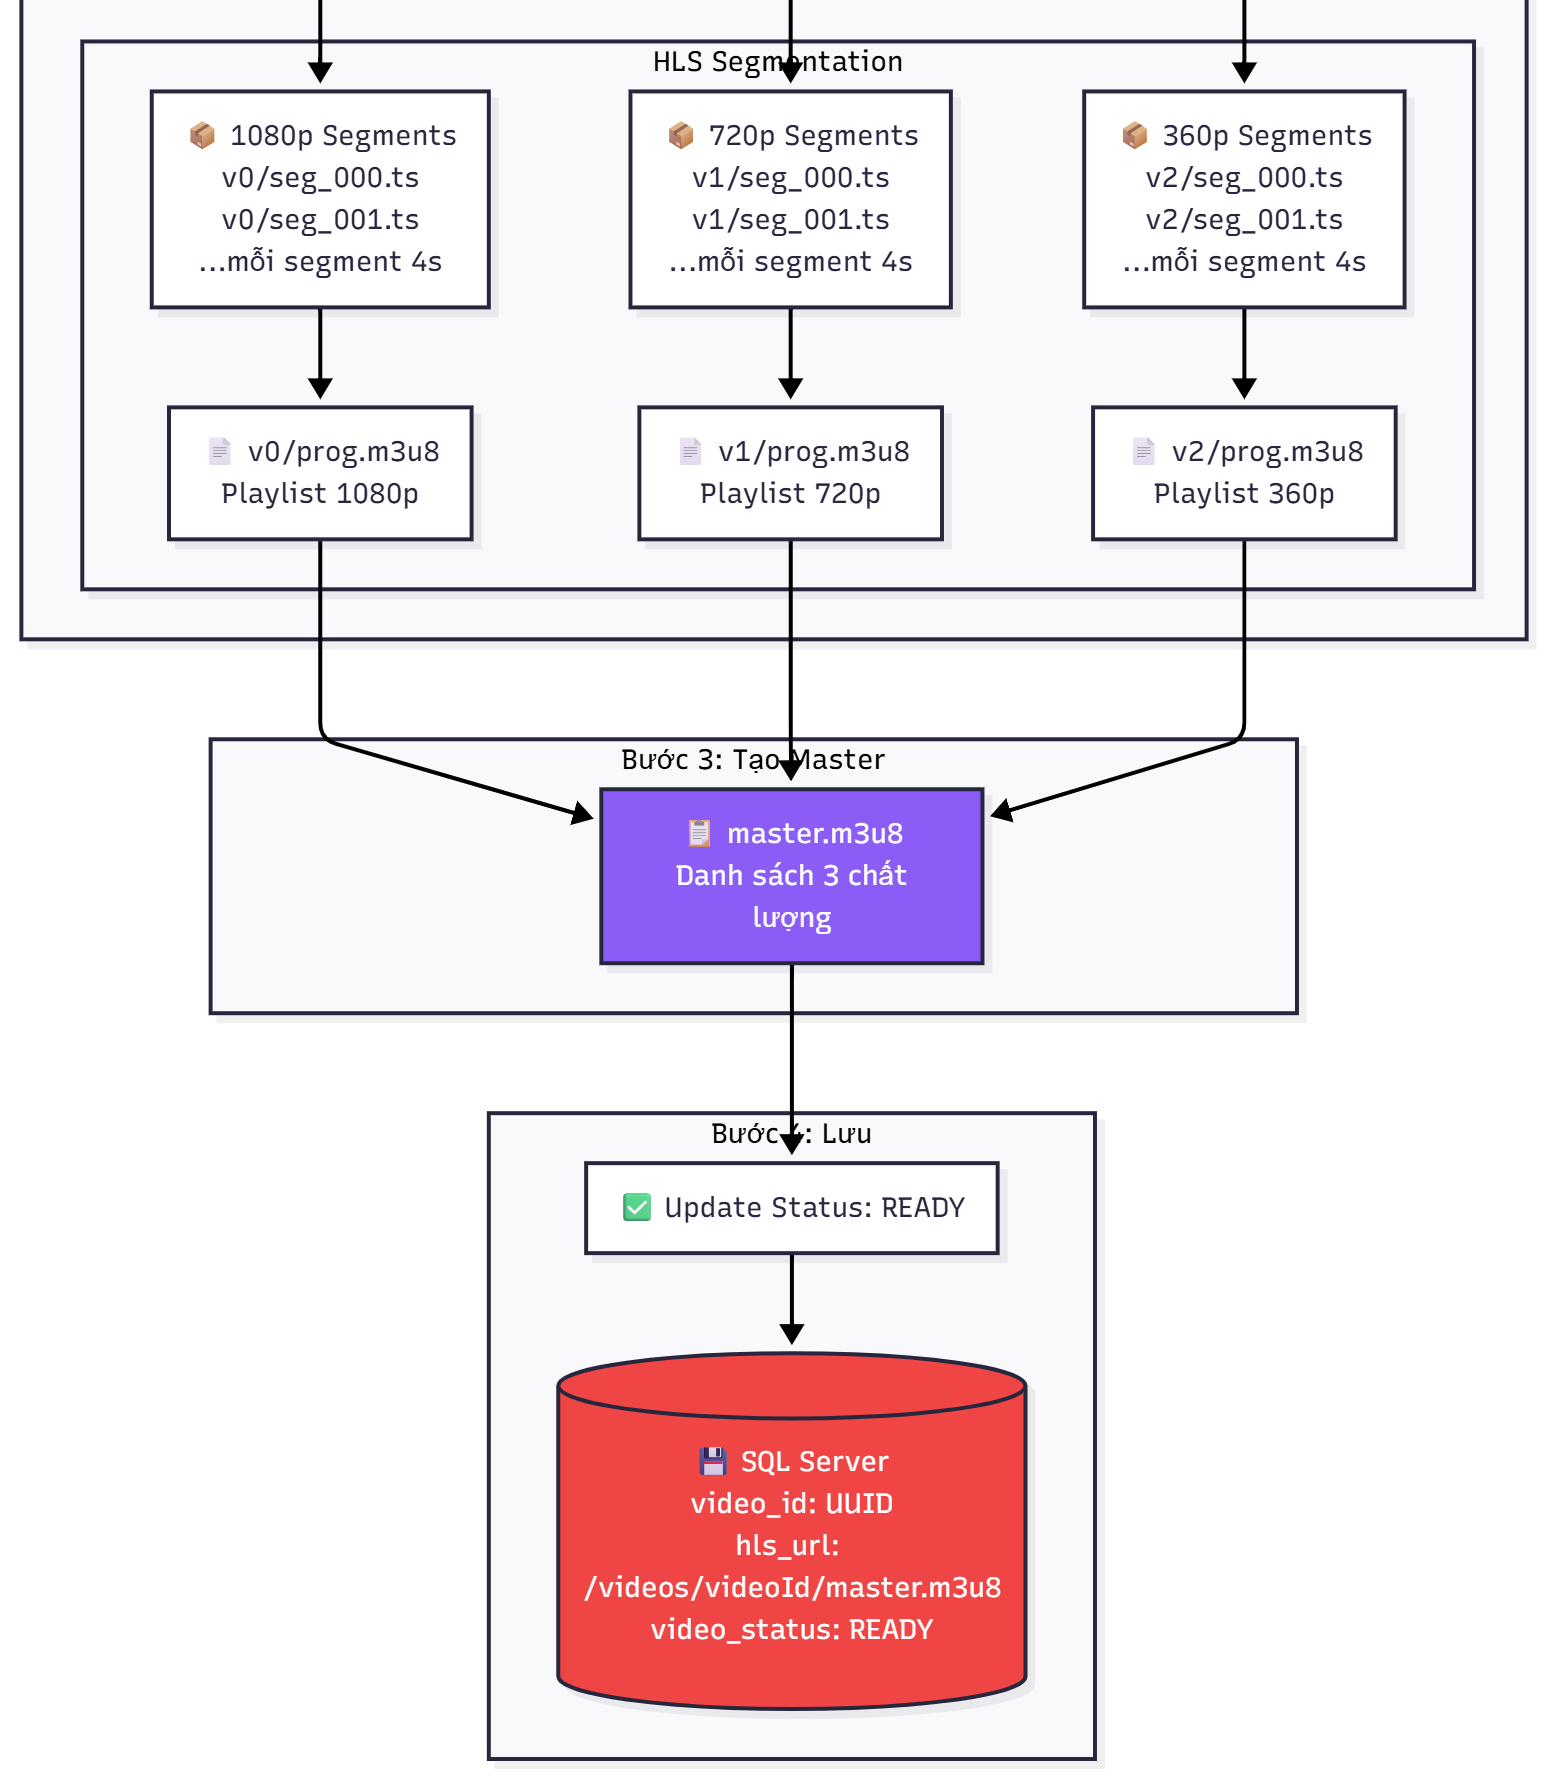
\includegraphics[width=1\textwidth]{image/mermaid/luongxulyvideo2.png}
	\caption{Luồng xử lý video trong hệ thống NicePhim}
	\label{fig:luongxulyvideo2}
\end{figure}

\subsection{Luồng phát video HLS}

\begin{figure}[H]
	\centering
	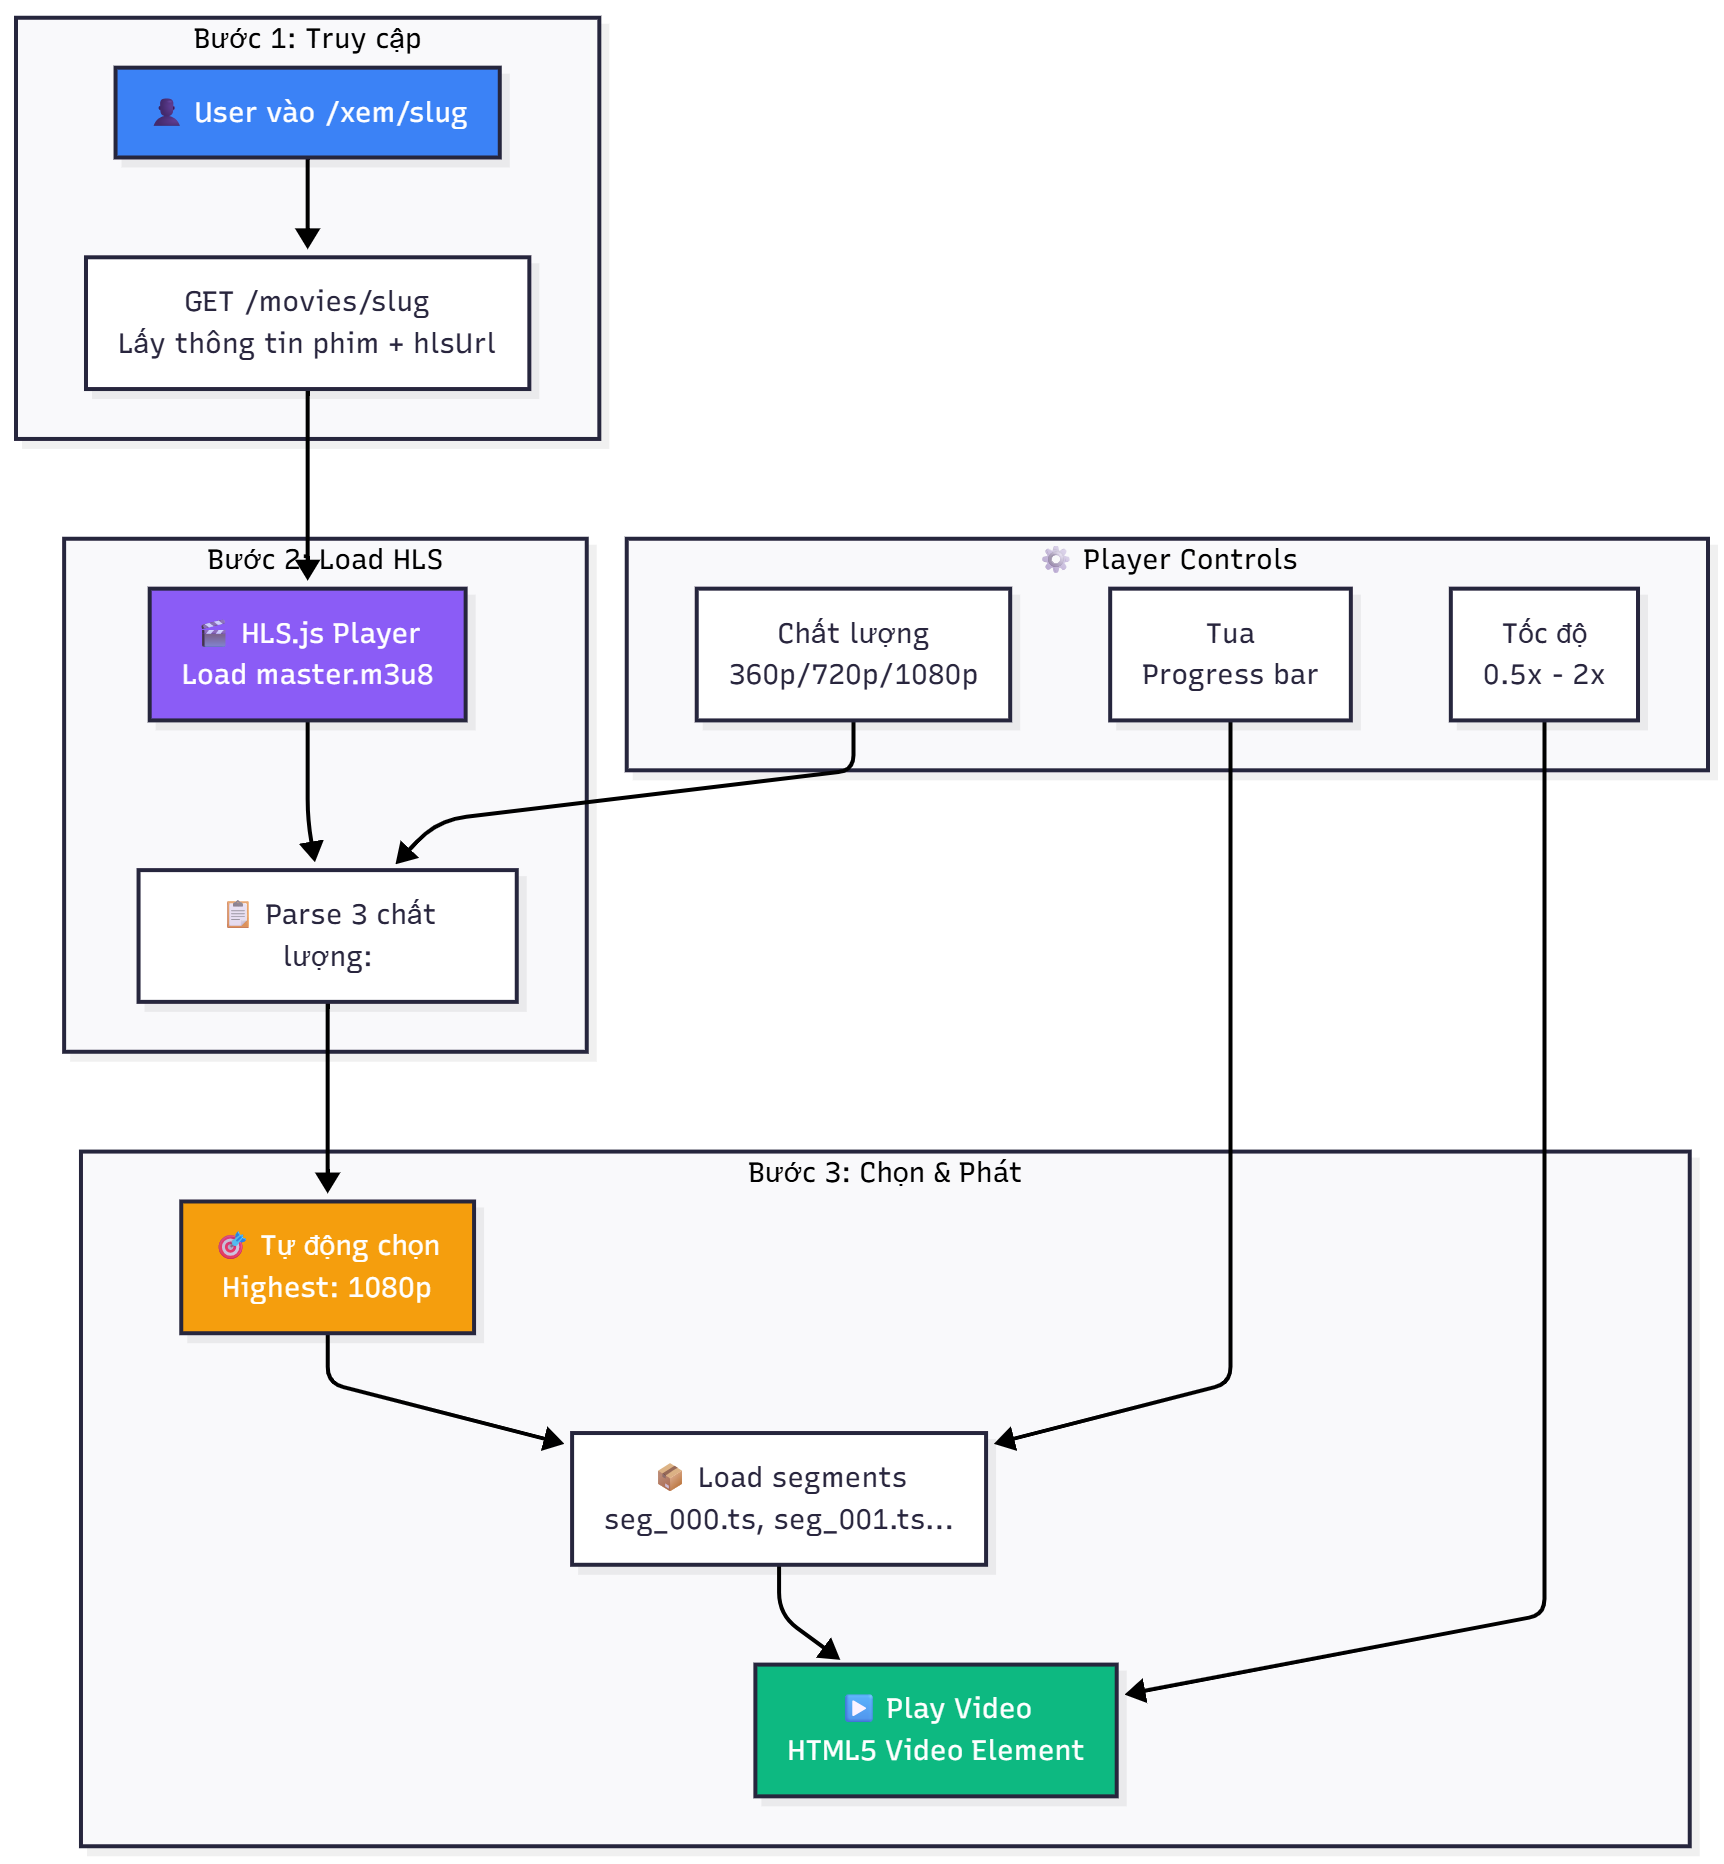
\includegraphics[width=1\textwidth]{image/mermaid/luongphatvideoHLS.png}
	\caption{Luồng phát video HLS trong hệ thống NicePhim}
	\label{fig:luongphatvideoHLS}
\end{figure}

\subsection{Luồng xem phim chung}

\begin{figure}[H]
	\centering
	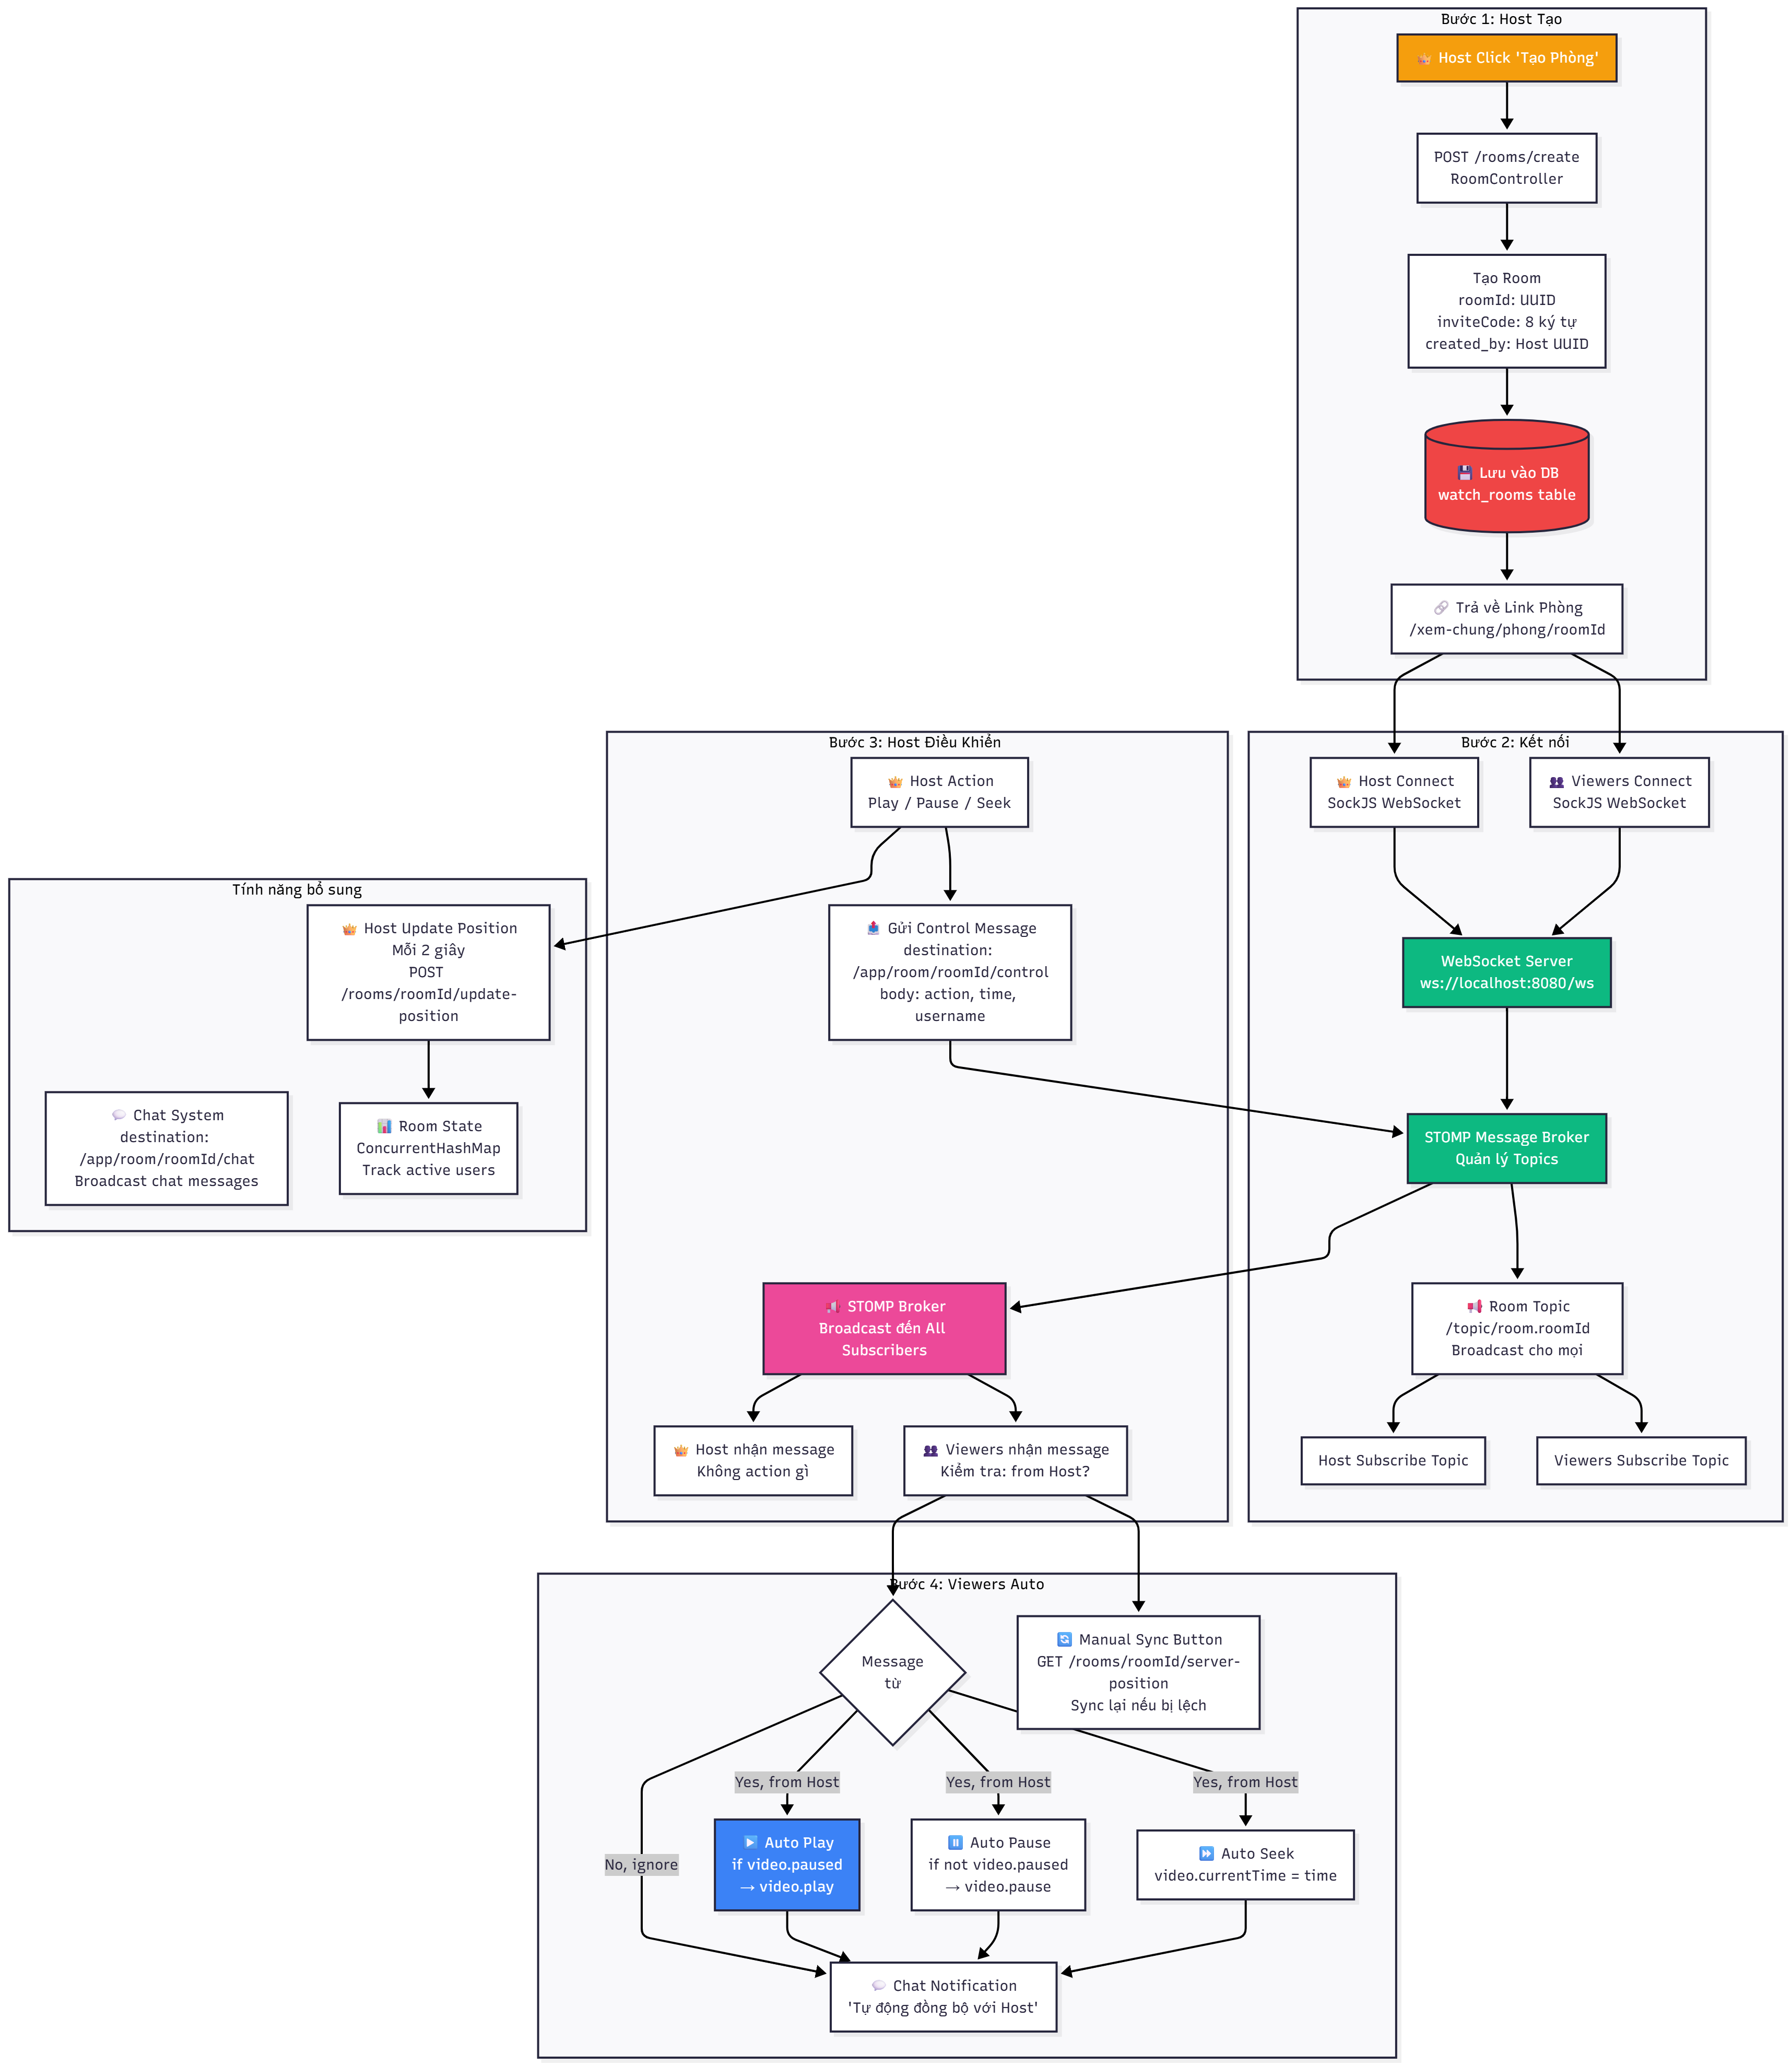
\includegraphics[width=1\textwidth]{image/mermaid/luongwatchtogether.png}
	\caption{Luồng xem phim chung trong hệ thống NicePhim}
	\label{fig:luongwatchtogether}
\end{figure}

\subsection{Luồng chat}

\begin{figure}[H]
	\centering
	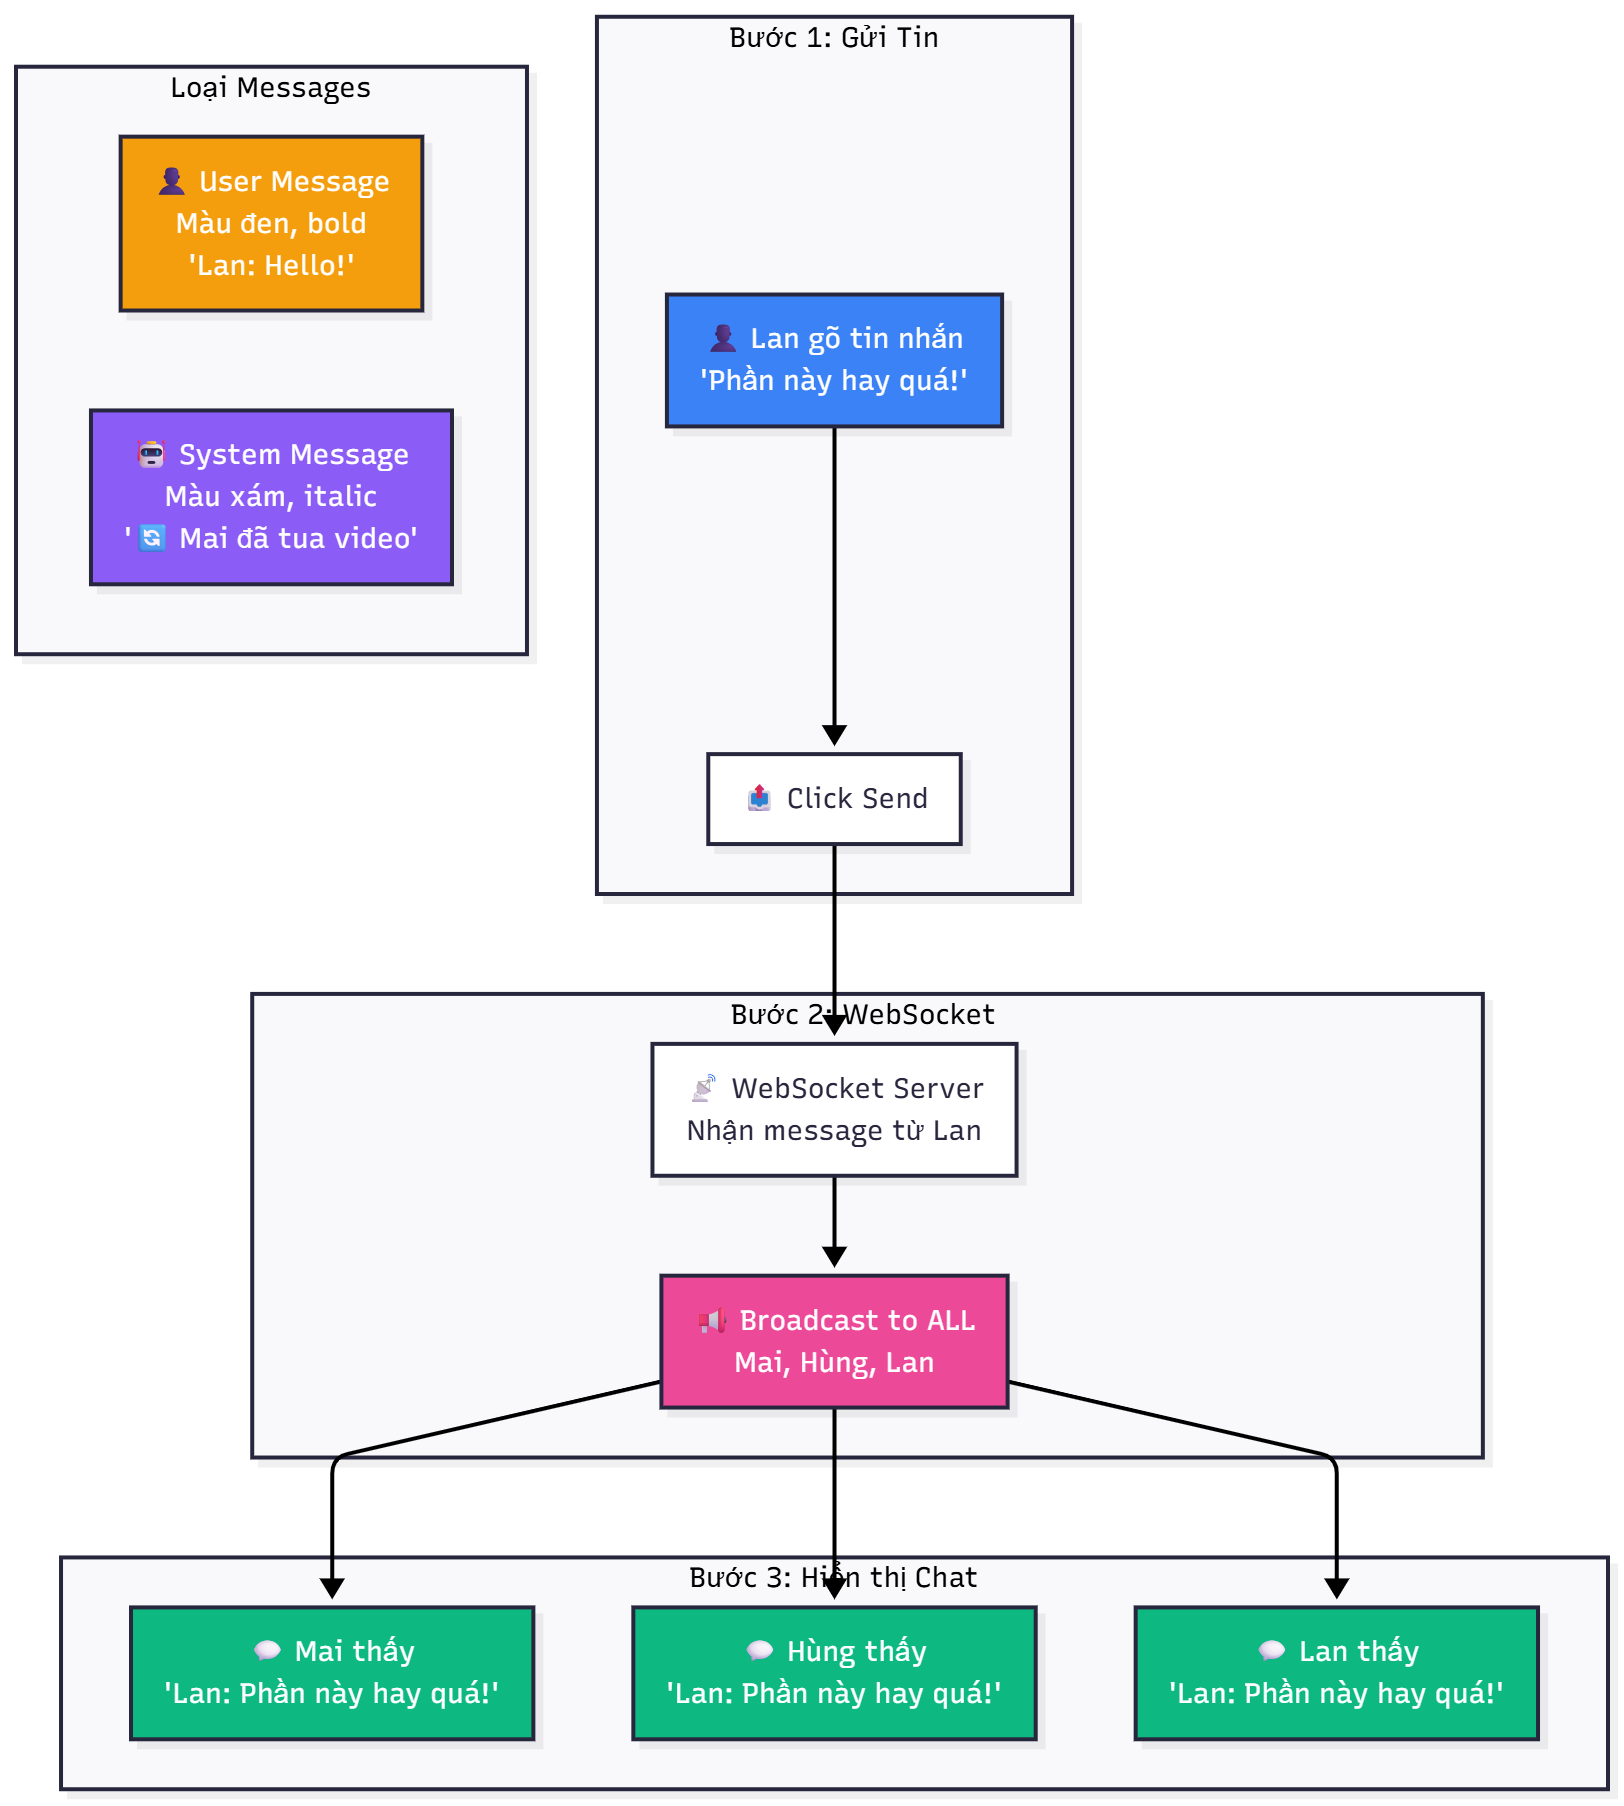
\includegraphics[width=1\textwidth]{image/mermaid/chat.png}
	\caption{Luồng chat trong hệ thống NicePhim}
	\label{fig:chat}
\end{figure}

\subsection{Cơ sở dữ liệu}

NicePhim sử dụng Microsoft SQL Server làm hệ quản trị cơ sở dữ liệu quan hệ. Database được thiết kế với 5 bảng chính để lưu trữ và quản lý dữ liệu của hệ thống. Các bảng được liên kết với nhau thông qua khóa ngoại (Foreign Key), đảm bảo tính toàn vẹn dữ liệu và hỗ trợ các truy vấn phức tạp. Tất cả các bảng sử dụng \texttt{uniqueidentifier} (UUID) làm khóa chính để đảm bảo tính duy nhất toàn cục và khả năng mở rộng.

Mối quan hệ giữa các bảng:
\begin{itemize}
	\item \textbf{users} tạo nhiều \textbf{movies} (1-nhiều)
	\item \textbf{users} tạo nhiều \textbf{watch\_rooms} (1-nhiều)
	\item \textbf{movies} thuộc nhiều \textbf{genres} thông qua bảng trung gian \textbf{movie\_genres} (nhiều-nhiều)
	\item \textbf{movies} được xem trong nhiều \textbf{watch\_rooms} (1-nhiều)
\end{itemize}

\subsubsection{Bảng users}

Bảng \texttt{users} lưu trữ thông tin người dùng của hệ thống, bao gồm thông tin xác thực và profile.

\begin{center}
	\small
	\begin{longtable}{|c|p{3.5cm}|p{2.5cm}|p{3cm}|p{3.5cm}|}
		\caption{Cấu trúc bảng users} \label{tab:users}                                                                     \\
		\hline
		\textbf{STT} & \textbf{Tên trường} & \textbf{Kiểu dữ liệu} & \textbf{Ràng buộc}       & \textbf{Mô tả}              \\
		\hline
		\endfirsthead

		\multicolumn{5}{c}%
		{{\tablename\ \thetable{} -- tiếp theo trang trước}}                                                                \\
		\hline
		\textbf{STT} & \textbf{Tên trường} & \textbf{Kiểu dữ liệu} & \textbf{Ràng buộc}       & \textbf{Mô tả}              \\
		\hline
		\endhead

		\hline \multicolumn{5}{r}{{Tiếp trang sau}}                                                                         \\
		\endfoot

		\hline
		\endlastfoot

		1            & user\_id            & uniqueidentifier      & PK                       & Mã định danh người dùng     \\
		\hline
		2            & username            & nvarchar(255)         & UK, NOT NULL             & Tên đăng nhập duy nhất      \\
		\hline
		3            & email               & nvarchar(255)         & UK, NOT NULL             & Địa chỉ email duy nhất      \\
		\hline
		4            & password\_hash      & varbinary(MAX)        & NOT NULL                 & Mật khẩu đã mã hóa BCrypt   \\
		\hline
		5            & display\_name       & nvarchar(255)         &                          & Tên hiển thị của người dùng \\
		\hline
		6            & avatar\_url         & nvarchar(500)         &                          & URL ảnh đại diện            \\
		\hline
		7            & is\_admin           & bit                   & DEFAULT 0                & Quyền quản trị viên         \\
		\hline
		8            & created\_at         & datetime2             & DEFAULT SYSUTCDATETIME() & Thời gian tạo tài khoản     \\
		\hline
		9            & updated\_at         & datetime2             &                          & Thời gian cập nhật cuối     \\
		\hline
	\end{longtable}
\end{center}

\subsubsection{Bảng movies}

Bảng \texttt{movies} lưu trữ thông tin chi tiết về các bộ phim trong hệ thống, bao gồm metadata và đường dẫn video.

\begin{center}
	\small
	\begin{longtable}{|c|p{3cm}|p{2.5cm}|p{3cm}|p{4cm}|}
		\caption{Cấu trúc bảng movies} \label{tab:movies}                                                                      \\
		\hline
		\textbf{STT} & \textbf{Tên trường} & \textbf{Kiểu dữ liệu} & \textbf{Ràng buộc}       & \textbf{Mô tả}                 \\
		\hline
		\endfirsthead

		\multicolumn{5}{c}%
		{{\tablename\ \thetable{} -- tiếp theo trang trước}}                                                                   \\
		\hline
		\textbf{STT} & \textbf{Tên trường} & \textbf{Kiểu dữ liệu} & \textbf{Ràng buộc}       & \textbf{Mô tả}                 \\
		\hline
		\endhead

		\hline \multicolumn{5}{r}{{Tiếp trang sau}}                                                                            \\
		\endfoot

		\hline
		\endlastfoot

		1            & movie\_id           & uniqueidentifier      & PK                       & Mã định danh phim              \\
		\hline
		2            & title               & nvarchar(255)         & NOT NULL                 & Tiêu đề phim                   \\
		\hline
		3            & alias\_title        & nvarchar(255)         &                          & Tiêu đề phụ hoặc tên gốc       \\
		\hline
		4            & description         & nvarchar(MAX)         &                          & Mô tả nội dung phim            \\
		\hline
		5            & release\_year       & smallint              &                          & Năm phát hành                  \\
		\hline
		6            & age\_rating         & nvarchar(10)          &                          & Giới hạn độ tuổi (PG, R, etc.) \\
		\hline
		7            & imdb\_rating        & decimal(3,1)          &                          & Điểm đánh giá IMDB             \\
		\hline
		8            & is\_series          & bit                   & DEFAULT 0                & Phân biệt phim lẻ/phim bộ      \\
		\hline
		9            & poster\_url         & nvarchar(500)         &                          & URL hình poster                \\
		\hline
		10           & banner\_url         & nvarchar(500)         &                          & URL hình banner                \\
		\hline
		11           & created\_by         & uniqueidentifier      & FK (users), NOT NULL     & Người tạo phim                 \\
		\hline
		12           & video\_id           & nvarchar(100)         &                          & ID video trong storage         \\
		\hline
		13           & hls\_url            & nvarchar(500)         &                          & URL manifest HLS (.m3u8)       \\
		\hline
		14           & video\_status       & nvarchar(20)          &                          & Trạng thái xử lý video         \\
		\hline
		15           & created\_at         & datetime2             & DEFAULT SYSUTCDATETIME() & Thời gian tạo                  \\
		\hline
		16           & updated\_at         & datetime2             &                          & Thời gian cập nhật cuối        \\
		\hline
	\end{longtable}
\end{center}

\subsubsection{Bảng genres}

Bảng \texttt{genres} lưu trữ danh sách các thể loại phim có trong hệ thống.

\begin{center}
	\small
	\begin{longtable}{|c|p{4cm}|p{3cm}|p{3cm}|p{4cm}|}
		\caption{Cấu trúc bảng genres} \label{tab:genres}                                                                    \\
		\hline
		\textbf{STT} & \textbf{Tên trường} & \textbf{Kiểu dữ liệu} & \textbf{Ràng buộc} & \textbf{Mô tả}                     \\
		\hline
		\endfirsthead

		\multicolumn{5}{c}%
		{{\tablename\ \thetable{} -- tiếp theo trang trước}}                                                                 \\
		\hline
		\textbf{STT} & \textbf{Tên trường} & \textbf{Kiểu dữ liệu} & \textbf{Ràng buộc} & \textbf{Mô tả}                     \\
		\hline
		\endhead

		\hline \multicolumn{5}{r}{{Tiếp trang sau}}                                                                          \\
		\endfoot

		\hline
		\endlastfoot

		1            & genre\_id           & uniqueidentifier      & PK                 & Mã định danh thể loại              \\
		\hline
		2            & name                & nvarchar(100)         & UK, NOT NULL       & Tên thể loại (Action, Drama, etc.) \\
		\hline
	\end{longtable}
\end{center}

\subsubsection{Bảng movie\_genres}

Bảng \texttt{movie\_genres} là bảng trung gian (junction table) thiết lập mối quan hệ nhiều-nhiều giữa \texttt{movies} và \texttt{genres}, cho phép một phim thuộc nhiều thể loại và một thể loại chứa nhiều phim.

\begin{center}
	\small
	\begin{longtable}{|c|p{4cm}|p{3cm}|p{3cm}|p{4cm}|}
		\caption{Cấu trúc bảng movie\_genres} \label{tab:movie_genres}                                          \\
		\hline
		\textbf{STT} & \textbf{Tên trường} & \textbf{Kiểu dữ liệu} & \textbf{Ràng buộc} & \textbf{Mô tả}        \\
		\hline
		\endfirsthead

		\multicolumn{5}{c}%
		{{\tablename\ \thetable{} -- tiếp theo trang trước}}                                                    \\
		\hline
		\textbf{STT} & \textbf{Tên trường} & \textbf{Kiểu dữ liệu} & \textbf{Ràng buộc} & \textbf{Mô tả}        \\
		\hline
		\endhead

		\hline \multicolumn{5}{r}{{Tiếp trang sau}}                                                             \\
		\endfoot

		\hline
		\endlastfoot

		1            & movie\_id           & uniqueidentifier      & PK, FK (movies)    & Mã định danh phim     \\
		\hline
		2            & genre\_id           & uniqueidentifier      & PK, FK (genres)    & Mã định danh thể loại \\
		\hline
	\end{longtable}
\end{center}

\textit{Lưu ý: Bảng này sử dụng composite primary key gồm cả movie\_id và genre\_id.}

\subsubsection{Bảng watch\_rooms}

Bảng \texttt{watch\_rooms} lưu trữ thông tin về các phòng xem chung, bao gồm trạng thái phát video được đồng bộ giữa các thành viên.

\begin{center}
	\small
	\begin{longtable}{|c|p{3cm}|p{2.5cm}|p{3.5cm}|p{4cm}|}
		\caption{Cấu trúc bảng watch\_rooms} \label{tab:watch_rooms}                                                                 \\
		\hline
		\textbf{STT} & \textbf{Tên trường} & \textbf{Kiểu dữ liệu} & \textbf{Ràng buộc}       & \textbf{Mô tả}                       \\
		\hline
		\endfirsthead

		\multicolumn{5}{c}%
		{{\tablename\ \thetable{} -- tiếp theo trang trước}}                                                                         \\
		\hline
		\textbf{STT} & \textbf{Tên trường} & \textbf{Kiểu dữ liệu} & \textbf{Ràng buộc}       & \textbf{Mô tả}                       \\
		\hline
		\endhead

		\hline \multicolumn{5}{r}{{Tiếp trang sau}}                                                                                  \\
		\endfoot

		\hline
		\endlastfoot

		1            & room\_id            & uniqueidentifier      & PK                       & Mã định danh phòng                   \\
		\hline
		2            & name                & nvarchar(255)         & NOT NULL                 & Tên phòng xem chung                  \\
		\hline
		3            & created\_by         & uniqueidentifier      & FK (users), NOT NULL     & Người tạo phòng                      \\
		\hline
		4            & movie\_id           & uniqueidentifier      & FK (movies)              & Phim đang xem trong phòng            \\
		\hline
		5            & current\_time\_ms   & bigint                & DEFAULT 0                & Vị trí video hiện tại (milliseconds) \\
		\hline
		6            & playback\_state     & tinyint               & DEFAULT 0                & Trạng thái phát (0: pause, 1: play)  \\
		\hline
		7            & playback\_rate      & decimal(3,2)          & DEFAULT 1.0              & Tốc độ phát (0.5x, 1x, 2x, etc.)     \\
		\hline
		8            & created\_at         & datetime2             & DEFAULT SYSUTCDATETIME() & Thời gian tạo phòng                  \\
		\hline
		9            & updated\_at         & datetime2             &                          & Thời gian cập nhật cuối              \\
		\hline
		10           & row\_version        & timestamp             &                          & Optimistic concurrency control       \\
		\hline
	\end{longtable}
\end{center}
